\documentclass[twocolumn]{article}
\usepackage[utf8]{inputenc}  % Soporte para caracteres UTF-8
\usepackage[spanish]{babel}  % Soporte para el idioma español
\usepackage{amsmath}
\usepackage{graphicx}
\usepackage{caption}
\usepackage{geometry}
\usepackage{hyperref}


\geometry{a4paper, margin=1in}

\title{Sonobiología: Un Enfoque en la Sonogenética Aplicada a Plantas}
\author{Sebastián Espinoza Domínguez//Jose Ledesma//David Ocaña//Brayan Rasca//Ruben Chavez}
\date{\today}

\begin{document}

\maketitle

\begin{abstract}
La sonobiología es un campo emergente que explora las interacciones entre el sonido y los organismos vivos. Este documento se centra en la sonogenética, una disciplina que estudia cómo las ondas sonoras pueden influir en la expresión genética de las plantas, ofreciendo nuevas oportunidades para la agricultura sostenible.
\end{abstract}

\section{Introducción}
La sonobiología se ocupa de la influencia del sonido en los sistemas biológicos. La sonogenética, una subdisciplina, investiga cómo las frecuencias sonoras pueden afectar la actividad genética. Este fenómeno ha despertado interés en la agricultura, donde se busca mejorar el crecimiento y la resistencia de las plantas.

\section{Principios de la Sonobiología}
La sonobiología se basa en la idea de que las ondas sonoras pueden inducir cambios en los procesos biológicos. Se ha demostrado que ciertas frecuencias son capaces de:

\begin{itemize}
    \item Estimular la germinación de semillas.
    \item Acelerar el crecimiento de las plantas.
    \item Aumentar la resistencia a enfermedades.
    \item Modificar la morfología de las plantas.
    \item Afectar procesos químicos específicos.
\end{itemize}

\begin{figure}[!h]
    \centering
    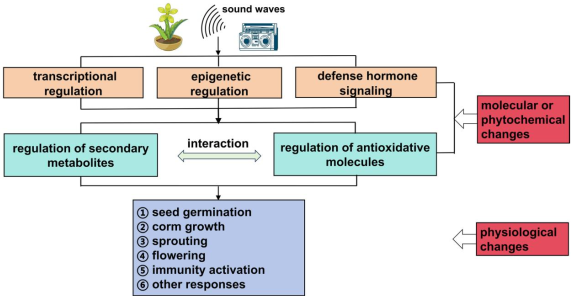
\includegraphics[width=\linewidth]{imagenes/Captura desde 2024-09-25 22-41-01.png}       
\end{figure}

\section{Sonogenética en Plantas}
La sonogenética se centra en la interacción entre el sonido y la expresión genética. Investigaciones recientes indican que esta tecnología no solo mejora las capacidades de las plantas, sino que también permite controlarlas o guiarlas, convirtiéndolas en herramientas para alcanzar metas específicas en la agricultura.

\subsection{Efectos del Sonido en la Expresión Génica}
Las ondas sonoras pueden activar o reprimir genes específicos en las plantas, lo que resulta en cambios en el fenotipo. Un ejemplo de esto es el elongamiento de las raíces.

\begin{figure}[!h]
    \centering
    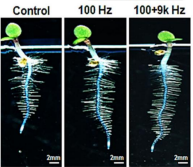
\includegraphics[width=\linewidth]{imagenes/Captura.PNG}
    \caption{Elongamiento de las raíces bajo la influencia de sonido.}
    \label{fig:elongamiento}
\end{figure}

\subsection{Métodos de Acción}
\begin{itemize}
    \item \textbf{Estrés en proteínas:} El estrés en las proteínas provoca que las moléculas no se estabilicen y no lleguen a donde deben.
    \begin{figure}[!h]
        \centering
        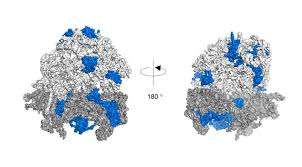
\includegraphics[width=\linewidth]{imagenes/descarga.jpeg}
        \caption{Estrés en proteínas.}
    \end{figure}
    
    \item \textbf{Ruptura Proteica:} Las moléculas de gran tamaño tienen una mayor mecanosensibilidad, lo que lleva a una mayor facilidad de ruptura. Esto resulta en:
    \begin{itemize}
        \item \textbf{Inhibición de la molécula:} Debido a la ruptura, se puede volver inservible a la molécula, evitando que cumpla su función.
        \begin{figure}[!h]
            \centering
            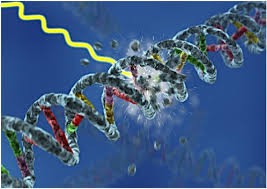
\includegraphics[width=\linewidth]{imagenes/descarga (1).jpeg}
            \caption{Inhibición de moléculas.}
        \end{figure}
        
        \item \textbf{Reducción Molecular:} La ruptura de una molécula mayor tiene como objetivo convertirla en otro compuesto aplicable a diferentes casos de uso.
        \begin{figure}[!h]
            \centering
            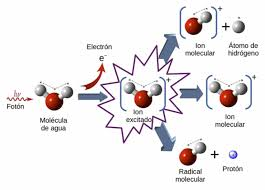
\includegraphics[width=\linewidth]{imagenes/descarga (4).jpeg}
            \caption{Reducción molecular.}
        \end{figure}
    \end{itemize}

    \item \textbf{Afectación a los canales iónicos intracelulares:} Este sistema permite manejar la entrada y salida de compuestos, tanto de nutrición como de señalización, regulando su velocidad.
    \begin{figure}[!h]
        \centering
        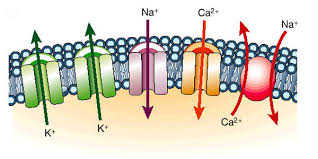
\includegraphics[width=\linewidth]{imagenes/descarga (5).jpeg}
        \caption{Afectación a los canales iónicos.}
    \end{figure}
    
    \item \textbf{Cavitación intercelular:} El sonido a alta frecuencia genera burbujas por cavitación, que son áreas de gas a alta temperatura, acelerando procesos metabólicos.
    \begin{figure}[!h]
        \centering
        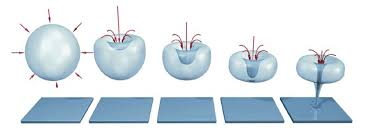
\includegraphics[width=\linewidth]{imagenes/images.jpeg}
        \caption{Cavitación intercelular.}
    \end{figure}
\end{itemize}

\subsection{Aplicaciones Prácticas}
\begin{itemize}
    \item Uso de frecuencias específicas para mejorar la calidad de cultivos.
    \begin{figure}[!h]
        \centering
        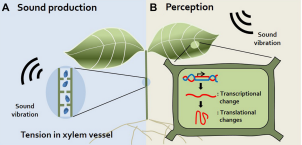
\includegraphics[width=\linewidth]{imagenes/Captura1.PNG}
        \caption{Uso de sonido para mejorar la calidad de cultivos.}
        \label{fig:calidad-cultivos}
    \end{figure}
    
    \item Implementación de técnicas de sonido en invernaderos.
    \begin{figure}[!h]
        \centering
        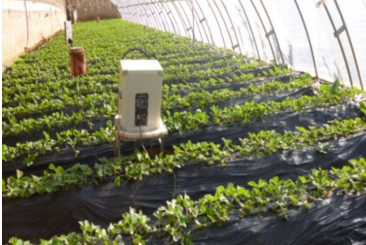
\includegraphics[width=\linewidth]{imagenes/Captura2.PNG}
        \caption{Implementación de técnicas de sonido en invernaderos.}
        \label{fig:invernaderos}
    \end{figure}
    
    \item Modificación del comportamiento o capacidades de las plantas.
    \begin{figure}[!h]
        \centering
        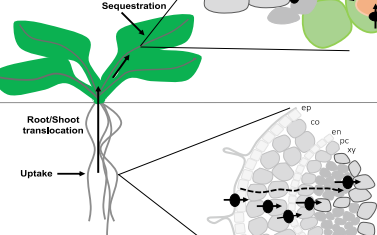
\includegraphics[width=\linewidth]{imagenes/Captura3.PNG}
        \caption{Modificación del comportamiento de las plantas por sonido.}
        \label{fig:modificacion}
    \end{figure}
\end{itemize}

\section{Mecanismos Moleculares Detrás de la Sonogenética}

La sonogenética se basa en la interacción entre las ondas sonoras y los procesos moleculares en las plantas.
 Comprender los mecanismos moleculares es crucial para aplicar efectivamente esta tecnología en la agricultura.
  A continuación, describiremos algunos de los mecanismos clave que se han identificado hasta ahora.

\subsection{Activación de Vías de Señalización}

Las ondas sonoras pueden inducir cambios en las vías de señalización celular, que son esenciales para la comunicación interna
 de las plantas. Estas vías pueden activarse o desactivarse en respuesta a estímulos acústicos, lo que lleva a cambios en la 
 expresión génica. Las proteínas quinasas, que actúan como mensajeros en estas vías, juegan un papel fundamental en la transducción
  de señales:

\begin{itemize}
    \item \textbf{Proteínas quinasas de mitógeno activadas (MAPK):} Estas proteínas son activadas por diversos estímulos,
     incluyendo el sonido. Una vez activadas, pueden fosforilar y regular la actividad de proteínas diana que influyen en el 
     crecimiento y desarrollo de las plantas.
    
    \item \textbf{Calcio como segundo mensajero:} Las oscilaciones en el calcio intracelular pueden ser inducidas por estímulos
     acústicos. Estas oscilaciones son señales críticas que pueden desencadenar respuestas celulares adaptativas.
\end{itemize}

\subsection{Modulación de la Expresión Génica}

La exposición a diferentes frecuencias sonoras puede afectar la transcripción de genes específicos, lo que se traduce
 en cambios fenotípicos en las plantas. Este proceso involucra:

\begin{figure}
    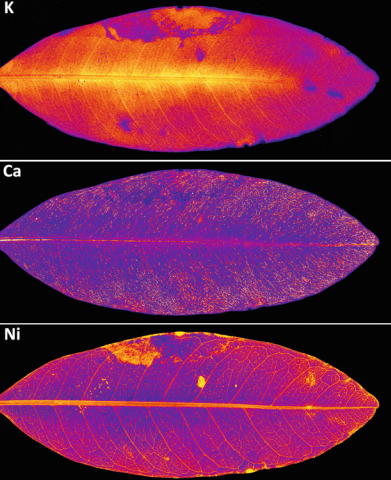
\includegraphics[width=\linewidth]{imagenes/Captura5.png}
\end{figure}

\begin{itemize}
    \item \textbf{Factores de transcripción:} Estas proteínas se unen a secuencias específicas de ADN para regular la expresión
     de genes. La activación de ciertos factores de transcripción por el sonido puede promover o inhibir la producción de proteínas
      involucradas en el crecimiento y desarrollo.
    
    \item \textbf{Metilación del ADN:} La modificación química del ADN puede ser influenciada por estímulos acústicos. 
    La metilación del ADN puede silenciar o activar genes, afectando la manera en que las plantas responden a su entorno.
\end{itemize}

\subsection{Respuesta a Estrés}

El sonido también puede inducir respuestas de estrés en las plantas, similar a otros factores ambientales como la sequía o el exceso de sal. Estas respuestas son mediadas por:

\begin{itemize}
    \item \textbf{Producción de proteínas de choque térmico:} Estas proteínas se producen en respuesta al estrés y ayudan a proteger las células. Se ha observado que las ondas sonoras pueden aumentar la expresión de HSP, mejorando la tolerancia de las plantas a condiciones adversas.
    
    \item \textbf{Antioxidantes:} El sonido puede estimular la producción de compuestos antioxidantes que protegen a las plantas del daño oxidativo, promoviendo la salud y el crecimiento en condiciones estresantes.
\end{itemize}

\subsection{Cambios en la Morfología y Fisiología}

Los cambios moleculares inducidos por el sonido pueden llevar a modificaciones en la morfología y fisiología de las plantas. Esto incluye:

\begin{itemize}
    \item \textbf{Elongación de raíces:} La exposición a ciertas frecuencias sonoras puede fomentar el crecimiento de raíces más largas y robustas, lo que aumenta la capacidad de las plantas para absorber agua y nutrientes.
    
    \item \textbf{Desarrollo foliar:} El sonido también puede influir en el tamaño y forma de las hojas, optimizando la fotosíntesis y, por ende, el crecimiento general de la planta.
\end{itemize}

\subsection{Perspectivas Futuras en la Investigación Molecular}

El entendimiento de los mecanismos moleculares detrás de la sonogenética es un campo en desarrollo. Las investigaciones futuras deberían enfocarse en:

\begin{itemize}
    \item \textbf{Estudios genómicos y transcriptómicos:} Analizar cómo las diferentes frecuencias afectan la expresión de un gran número de genes simultáneamente, utilizando técnicas como la secuenciación de ARN para identificar patrones de expresión en respuesta a estímulos acústicos.
    
    \item \textbf{Interacción con otros factores ambientales:} Investigar cómo el sonido interactúa con otros factores como la luz, la temperatura y la humedad para determinar la mejor manera de aplicar la sonogenética en entornos agrícolas reales.
\end{itemize}

Comprender los mecanismos moleculares de la sonogenética no solo ayuda a optimizar el crecimiento de las plantas, sino que también puede ofrecer soluciones innovadoras para los desafíos agrícolas actuales y futuros.


\section{Estudios de Caso}
Varios estudios han mostrado resultados prometedores. Por ejemplo, se ha investigado la actividad de las raíces y el contenido de proteínas solubles. Otro uso interesante es en la fitominería, que consiste en el uso de plantas superacumuladoras para la recolección de minerales y recursos del suelo, donde la sonogenética permite regular la toma de estos compuestos y la generación de energía a partir de ellos.

\subsection{Fitominería}
La fitominería se refiere a la obtención o minería de recursos del suelo mediante plantas. Como se sabe, uno de los componentes clave en la nutrición de las plantas son los minerales en el suelo. Las plantas superacumuladoras absorben cantidades mucho mayores de minerales, lo que permite que los recursos sean extraídos de dos formas:

\begin{itemize}
    \item \textbf{Cremación:} Se recolecta toda la biomasa de las zonas de mayor concentración, es decir, hojas, tallos y ramas, y se incineran, dejando solo los minerales para su posterior recolección.
    \begin{figure}[!h]
        \centering
        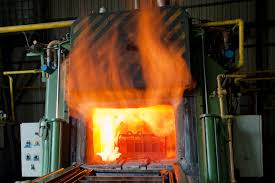
\includegraphics[width=\linewidth]{imagenes/descarga (6).jpeg}
        \caption{Cremación de biomasa para extracción de minerales.}
    \end{figure}
    
    \item \textbf{Bioreactores:} Se recolectan los productos desechados por el propio árbol, como hojas o ramas, los cuales son depositados en cilindros con microorganismos, principalmente bacterias, que separan los elementos deseados de forma limpia. 
    \begin{figure}[!h]
        \centering
        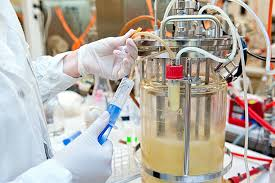
\includegraphics[width=\linewidth]{imagenes/descarga (7).jpeg}
        \caption{Bioreactores para separación de minerales.}
    \end{figure}
\end{itemize}

\subsection{Generación de Energía}
Las plantas se alimentan utilizando los nutrientes del suelo y el carbono del aire, usando el sol como fuente de energía. Lo que no consumen, lo desechan a través de sus raíces, donde microorganismos, como hongos o bacterias, los descomponen, liberando electrones y generando voltaje. Aunque la energía de una sola planta es insignificante, en un bosque entero, se pueden generar cantidades notables de energía. Algunas empresas ya están extrayendo energía de plantas, y otras venden pequeños dispositivos que funcionan completamente a partir de esta energía.
\begin{figure}[!h]
    \centering
    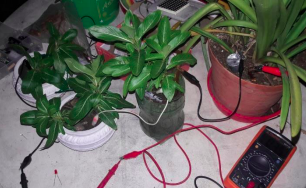
\includegraphics[width=\linewidth]{imagenes/Captura desde 2024-09-25 16-34-23.png}
    \caption{Generación de energía a partir de plantas.}
\end{figure}

\subsection{Sensores biológicos:}mas alla del uso de proteínas organicas para indicar una u otra cosa que se ha echo desde hace milenios
ahora se puede usar una planta en su completa existencia como identificador de cientos de parametros pH,calidad del aire,iluminacion e incluso olores
como ejemplo muesto un experimento echo por mi mismo:
\begin{figure}
    \centering
    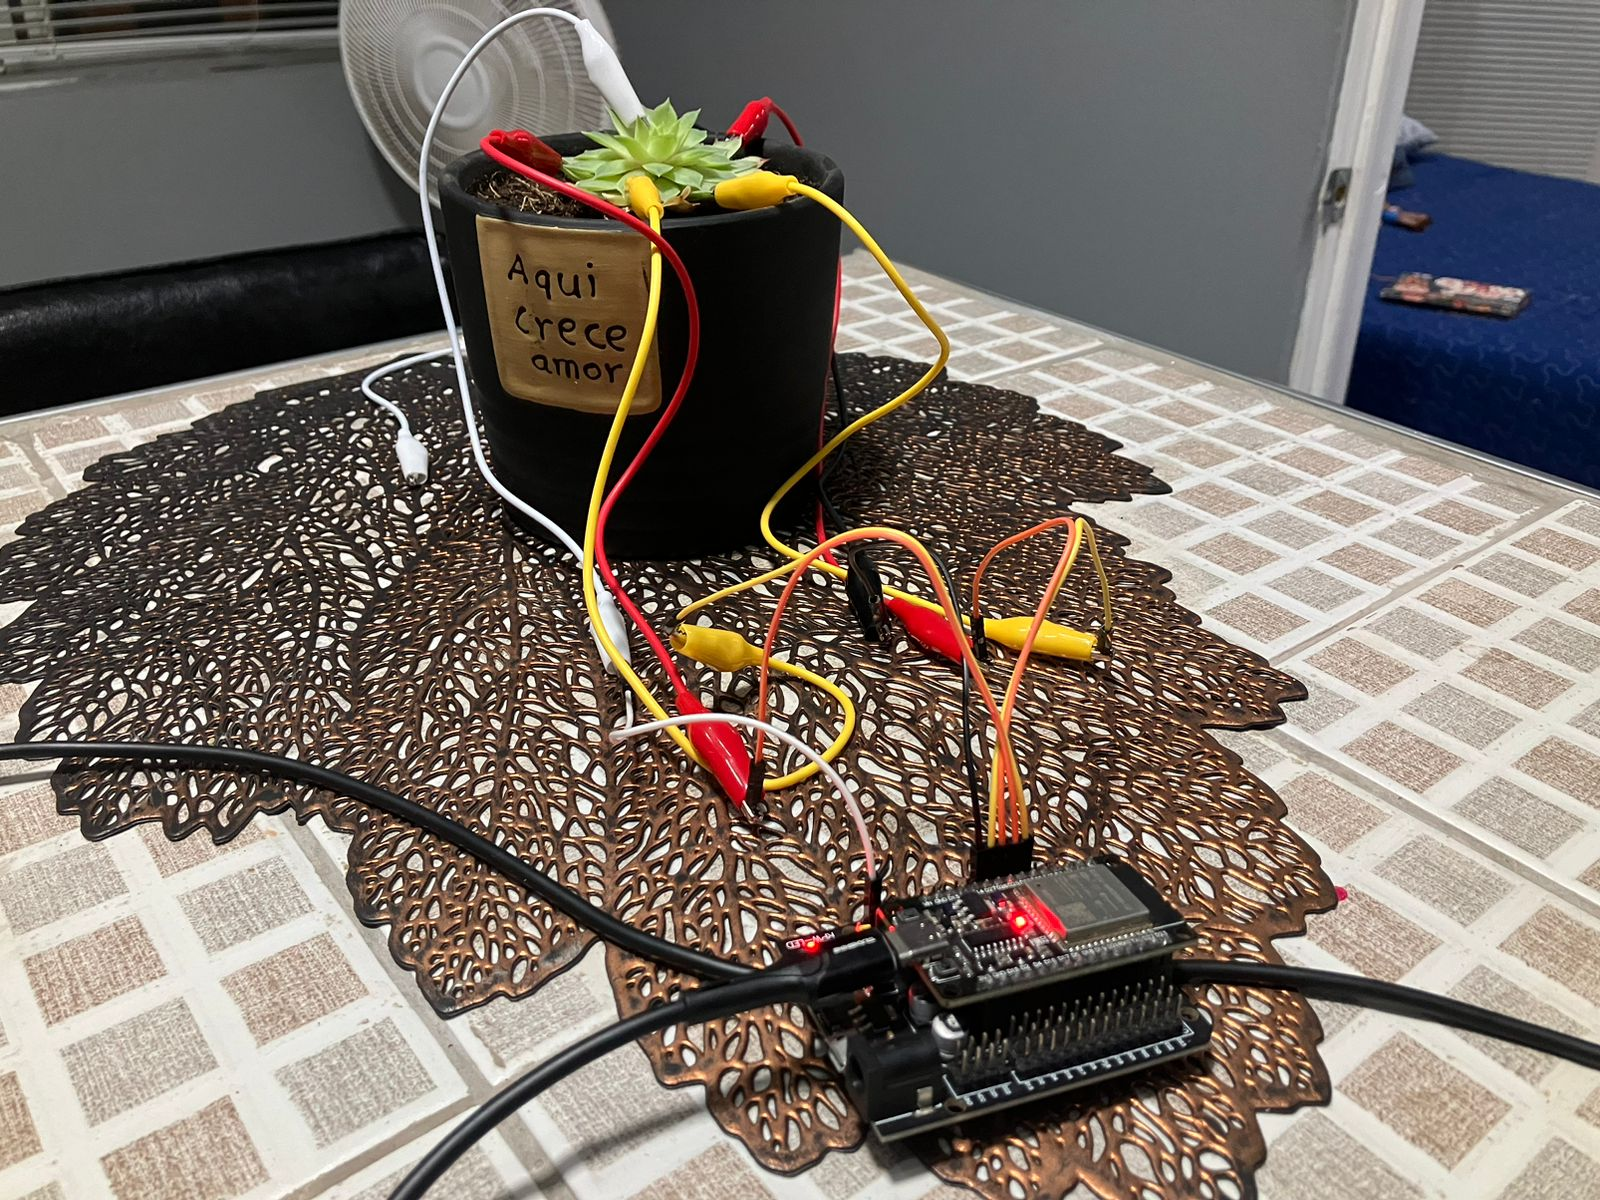
\includegraphics[width=\linewidth]{imagenes/b2600f88-8219-4305-a7c7-ee62c7193031.jpeg}
\end{figure}

\begin{figure}
    \centering
    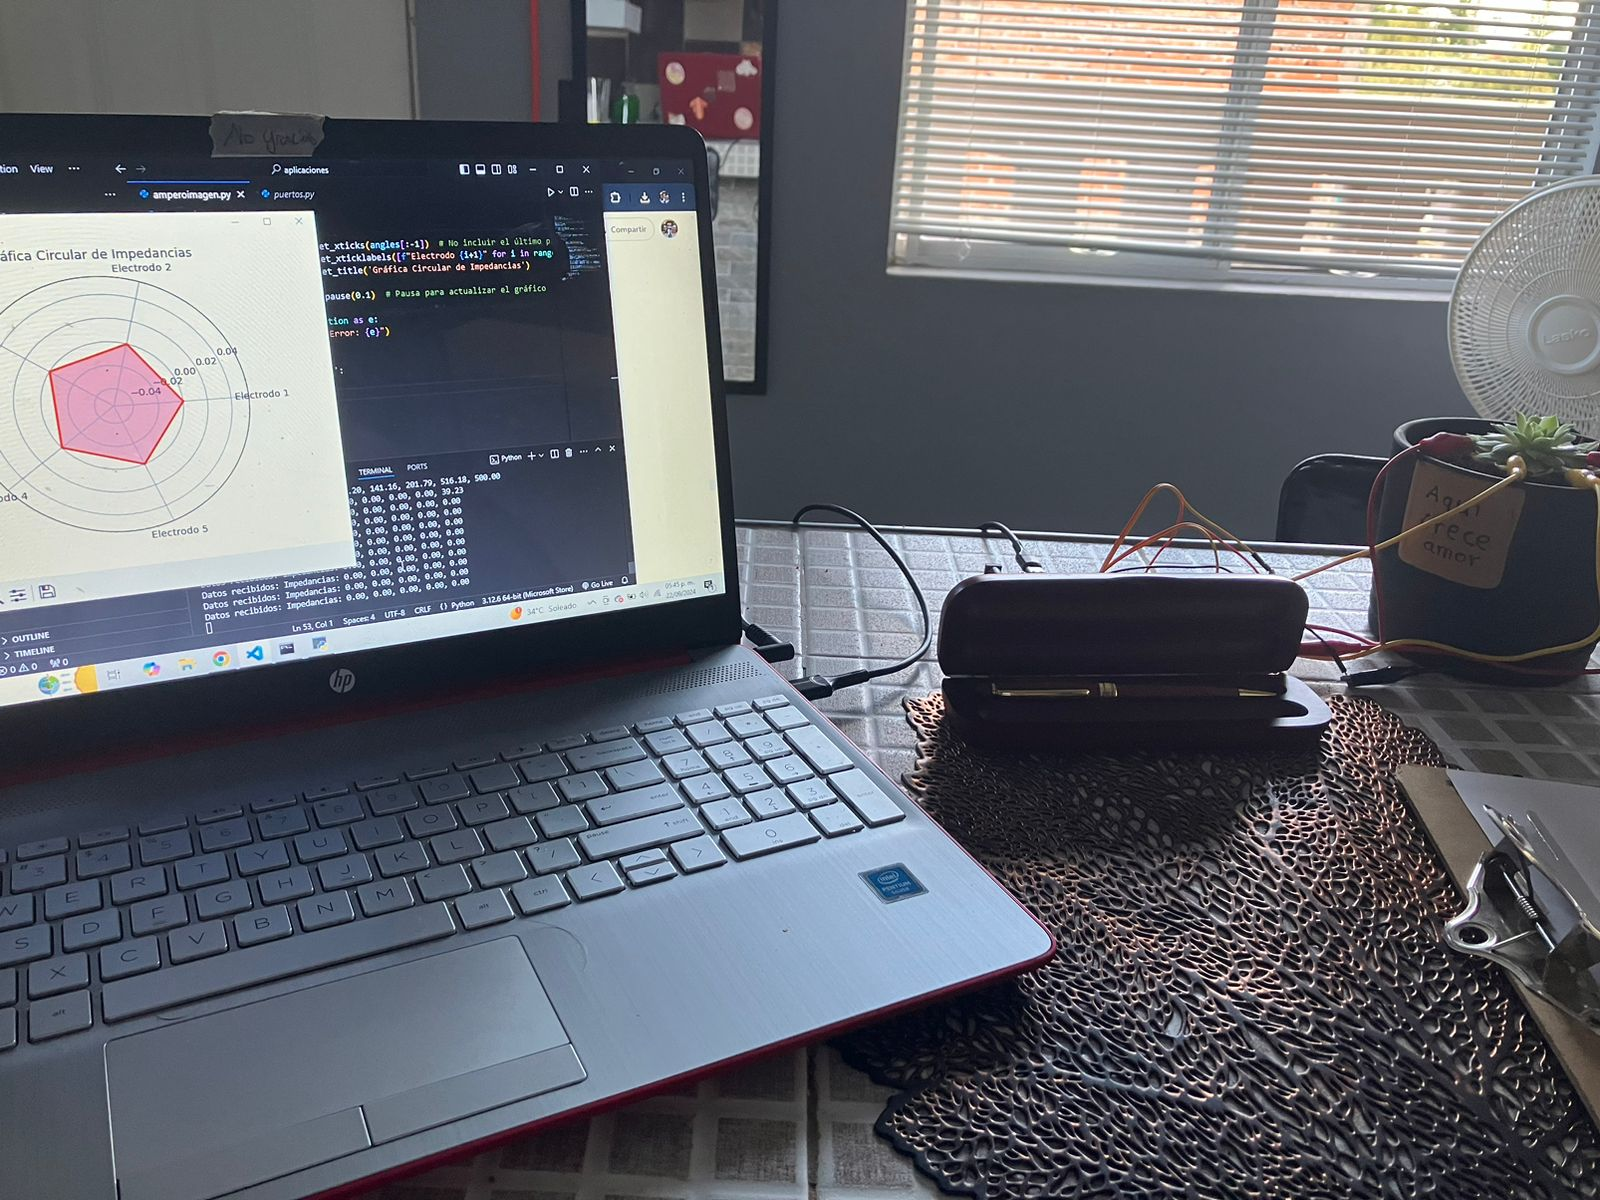
\includegraphics[width=\linewidth]{imagenes/2345deaa-69d8-4df1-ac8e-003b1e7546ac.jpeg}
\end{figure}
lo que se ve aqui en un sencillo programa para detectar las respuestas electricas de las plantas
ante distintos estimulos
\subsubsection{En que se relaciona con la sonogenetica?}las plantas se comunican de multiples maneras
de forma principal a esta investigacion el sonido especialmente ultrasonido 
\begin{figure}
    \centering
    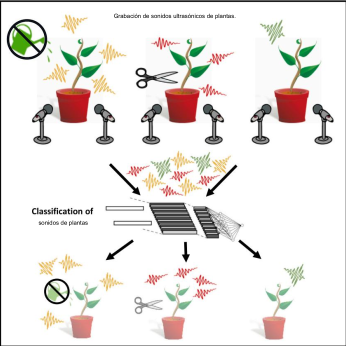
\includegraphics[width=\linewidth]{imagenes/Captura desde 2024-09-25 20-28-13.png}
\end{figure}
asi pues aqui podemos ver datos recolectados en una investigacion sobre la comunicacion vegetal \cite{khait2023sounds}
\begin{figure}
    \centering
    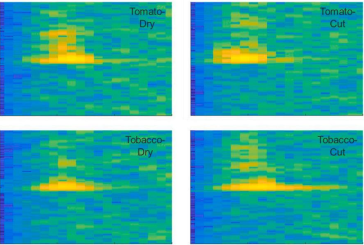
\includegraphics[width=\linewidth]{imagenes/Captura desde 2024-09-25 20-28-50.png}
\end{figure}
esto para alertar a otras plantas
de peligros,falta de nutrientes,plagas hasta para ponerse de acuerdo en la distribucion,las plantas 
al verse atacadas por insectos o ciertos tipos de animales emiten frecuencias no solo para avisar a otras plantas
del peligro sino tambien para llamar a los depredadores de estas.Pues retomando el tema original captando el habla/frecuencia 
de nuestra planta de interes podemos ver o escuchar a distancia las respuestas a estos estimulos

\section{Usos mas conocidos}
Durante esta investigación nos centraremos en un par de cosas para demostrar usos de esta tecnología
\begin{itemize}
    \item \textbf{Germinación:}La germinación es una de las etapas más críticas en el cultivo de plantas, y los agricultores enfrentan desafíos significativos debido a la baja tasa de éxito en la supervivencia de las semillas. La aplicación de tecnología sonora ha demostrado aumentar notablemente el índice de supervivencia de las semillas a un costo de recursos muy bajo, lo que a su vez reduce el estrés de los agricultores \cite{vicient2017}.
\begin{figure}[!h]
    \centering
    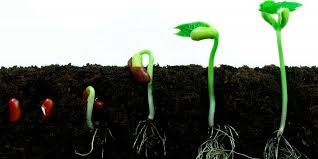
\includegraphics[width=\linewidth]{imagenes/descarga (9).jpeg}       
\end{figure}

\item \textbf{Crecimiento:}La estimulación celular provocada por las ondas sonoras impacta positivamente en el metabolismo de las plantas, acelerando la división celular y, por ende, aumentando su crecimiento y masa orgánica \cite{collins2001effect}.
\begin{figure}[!h]
    \centering
    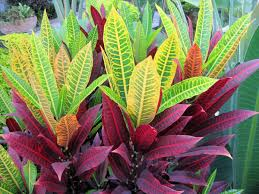
\includegraphics[width=\linewidth]{imagenes/images (2).jpeg}       
\end{figure}

\item \textbf{pH:}La lluvia ácida afecta gravemente la salud de los cultivos, provocando cambios en el pH del suelo que pueden resultar letales. Mediante el uso de sonogenética, es posible modificar los mecanismos naturales de las plantas de forma consciente para que puedan sobrevivir a estos cambios bruscos, activando o eliminando rutas de señalización específicas \cite{altuntas2019tomato}.
\begin{figure}[!h]
    \centering
    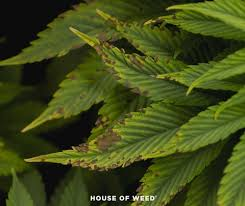
\includegraphics[width=\linewidth]{imagenes/images (3).jpeg}       
\end{figure}

\item \textbf{Metabolismo:} Esta tecnología también influye en la manera en que las plantas procesan sus nutrientes, acelerando o desacelerando estos procesos según las condiciones climáticas. Esto permite a las plantas aumentar su masa o reservar nutrientes mientras esperan un entorno más favorable \cite{Ozkurt2016}.
\begin{figure}[!h]
    \centering
    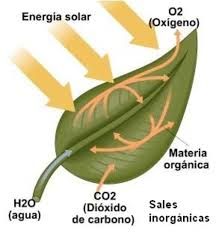
\includegraphics[width=\linewidth]{imagenes/descarga (8).jpeg}       
\end{figure}

\item \textbf{Coloración:} Existen tres métodos principales para modificar la coloración de las plantas a través de la sonogenética:

\subitem \textbf{Mecanosensibilidad de los pigmentos:} Esta técnica consiste en estresar los pigmentos para obtener colores más claros o diferentes de los originales, frecuentemente resultando en tonalidades blanquecinas.
    
\subitem \textbf{Efecto de cascada:} Este método más complejo requiere un profundo conocimiento de las rutas metabólicas intercelulares, ya que se basa en modificar las moléculas clave responsables del color en lugar de cambiar el resultado final.

\subitem \textbf{Modificación del pH y sus efectos en la coloración:} Utilizando lo aprendido sobre la regulación del pH, este método busca afectar los procesos clave que determinan el color de las plantas. Sin embargo, presenta limitaciones, como un rango de colores reducido y su dependencia directa de la salud de la planta \cite{altuntas2019tomato}, \cite{Rakic2021}.

\begin{figure}[!h]
    \centering
    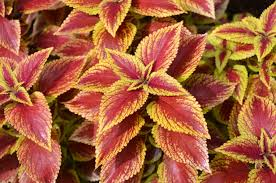
\includegraphics[width=\linewidth]{imagenes/images (1).jpeg}       
\end{figure}

\item \textbf{Fisiologia:} La sonogenética también puede modificar la densidad del tallo y la forma de las hojas. Esto se debe a la capacidad de regular los procesos de estrés, como la absorción de nutrientes, y permite a las plantas ajustar su dirección de crecimiento en respuesta a señales comunicativas de otras plantas.
\begin{figure}[!h]
    \centering
    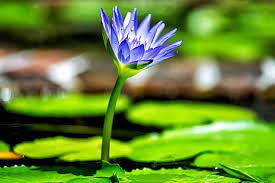
\includegraphics[width=\linewidth]{imagenes/images (4).jpeg}       
\end{figure}

\item \textbf{Raices:} La aplicación de esta tecnología puede afectar la profundidad, grosor, dispersión y arraigamiento de las raíces, lo que resulta esencial no solo para asegurar la producción de alimentos, sino también para emplear las plantas como máquinas industriales en tecnologías como la fitominería.
\begin{figure}[!h]
    \centering
    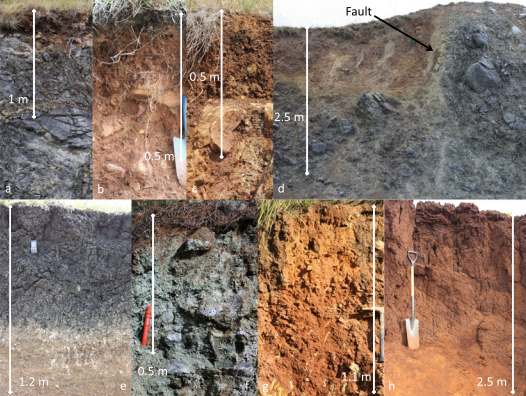
\includegraphics[width=\linewidth]{imagenes/Captura6.png}       
\end{figure}

\end{itemize}

\section{Impacto Ambiental y Sostenibilidad}

El uso de la sonogenética en plantas ofrece un potencial significativo para mejorar la agricultura sostenible, al aprovechar las interacciones entre las ondas sonoras y los organismos vegetales. Sin embargo, como cualquier tecnología emergente, es importante evaluar su impacto ambiental tanto desde una perspectiva de **beneficios** como de **riesgos potenciales**.

\subsection{Reducción de insumos agrícolas}

Uno de los principales beneficios ambientales de la sonogenética es la posibilidad de reducir la dependencia de insumos agrícolas convencionales, como fertilizantes químicos y pesticidas. Mediante la manipulación genética inducida por sonido, se pueden activar en las plantas mecanismos naturales de defensa contra plagas y enfermedades, lo que puede disminuir significativamente el uso de productos químicos tóxicos.

\begin{itemize}
    \item \textbf{Menor uso de pesticidas:} La estimulación sonora puede mejorar la resistencia natural de las plantas frente a insectos o patógenos. Esto no solo reduce el uso de pesticidas, sino que también protege los ecosistemas y la biodiversidad, ya que los pesticidas a menudo afectan a especies no objetivo como insectos polinizadores o predadores naturales.
    \begin{figure}[!h]
        \centering
        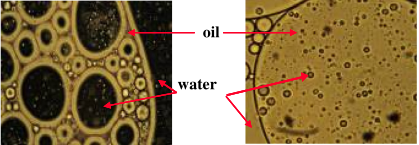
\includegraphics[width=\linewidth]{imagenes/Captura desde 2024-09-25 22-48-30.png}       
    \end{figure}
    \item \textbf{Optimización de nutrientes:} La mejora en la captación de nutrientes a través de la sonogenética puede reducir la necesidad de fertilizantes químicos, los cuales suelen lixiviarse en los cuerpos de agua, provocando \textit{eutrofización} (exceso de nutrientes que daña los ecosistemas acuáticos).
    \begin{figure}[!h]
        \centering
        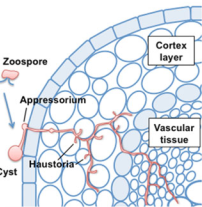
\includegraphics[width=\linewidth]{imagenes/Captura desde 2024-09-25 22-31-44.png}       
    \end{figure}
\end{itemize}

\subsection{Uso eficiente del agua}

Otra contribución ambiental clave de la sonogenética es su capacidad para optimizar el \textbf{uso del agua en los cultivos}. Mediante la manipulación genética sonora, es posible mejorar la eficiencia del uso de agua por parte de las plantas, lo que resulta crucial en áreas afectadas por la sequía.

\begin{itemize}
    \item \textbf{Tolerancia a la sequía:} Se ha demostrado que las plantas tratadas con determinadas frecuencias de sonido pueden desarrollar una mayor \textit{tolerancia al estrés hídrico}. Esto permite mantener la producción agrícola en regiones con recursos hídricos limitados, reduciendo así la presión sobre los acuíferos y otras fuentes de agua.
\end{itemize}

\subsection{Mitigación del cambio climático}

La sonogenética tiene el potencial de ayudar a mitigar los efectos del \textbf{cambio climático} mediante la creación de plantas más resistentes a condiciones ambientales extremas, como olas de calor o variaciones en los niveles de precipitación.

\begin{itemize}
    \item \textbf{Secuestro de carbono:} Mediante la modificación genética inducida por sonido, se pueden desarrollar plantas con mayor capacidad para almacenar carbono en sus raíces y suelos. Esto puede contribuir a los esfuerzos globales por reducir las concentraciones de dióxido de carbono en la atmósfera, un factor clave en la lucha contra el cambio climático.
\end{itemize}

\begin{figure}[!h]
    \centering
    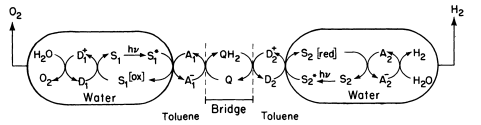
\includegraphics[width=\linewidth]{imagenes/Captura desde 2024-09-25 22-45-27.png}       
\end{figure}

\subsection{Minimización de la degradación del suelo}

El uso de tecnologías sonogenéticas puede también ayudar a minimizar la \textbf{degradación del suelo}. En muchas áreas agrícolas, el uso intensivo de fertilizantes y el riego excesivo han agotado los nutrientes del suelo y contribuido a la salinización. Mediante la sonogenética, se puede mejorar la capacidad de las plantas para acceder a nutrientes profundos y utilizar eficientemente los minerales disponibles, lo que podría reducir la necesidad de prácticas agrícolas dañinas para el suelo.


\subsection{Perspectiva para la sostenibilidad}

A medida que la investigación en sonogenética avanza, su implementación adecuada puede ofrecer soluciones sostenibles a muchos de los desafíos globales de la agricultura moderna. Al optimizar los recursos y reducir el impacto ambiental negativo de las prácticas agrícolas convencionales, la sonogenética puede contribuir a la creación de un \textbf{sistema agrícola más resiliente y respetuoso con el medio ambiente}.

Sin embargo, es importante abordar con precaución cualquier aplicación a gran escala y asegurarse de que las intervenciones tecnológicas no produzcan efectos adversos no deseados sobre el ecosistema. El desarrollo de \textbf{normativas ambientales claras} y una evaluación continua del impacto ambiental serán factores clave para garantizar que esta tecnología se use de manera ética y responsable.



\section{Desarrollo de Tecnología y Dispositivos Acústicos}

El avance de la sonobiología y la sonogenética ha sido impulsado en gran medida por el desarrollo de tecnologías y dispositivos acústicos innovadores. Estos dispositivos permiten aplicar y medir con precisión las ondas sonoras en entornos agrícolas y de investigación, facilitando el estudio de sus efectos en las plantas y optimizando su uso en prácticas agrícolas sostenibles.

\subsection{Dispositivos de Generación de Sonido}

Existen varios tipos de dispositivos diseñados para generar ondas sonoras específicas que pueden ser utilizadas en estudios de sonobiología. Estos dispositivos pueden clasificarse en dos categorías principales:

\begin{itemize}
    \item \textbf{Transductores:} Estos dispositivos convierten señales eléctricas en ondas sonoras. Pueden ser utilizados para generar frecuencias específicas que afectan a las plantas. Los transductores piezoeléctricos y los altavoces de rango amplio son ejemplos comunes que se utilizan en investigaciones sobre sonobiología.
    \begin{figure}[!h]
        \centering
        
\includegraphics[width=\linewidth]{imagenes/1faee7cd-2d65-47b5-9463-7e09d6f5016d.jpeg}       
    \end{figure}
    \item \textbf{Generadores de Frecuencia:} Estos dispositivos crean frecuencias sonoras ajustables que se pueden utilizar en experimentos. Los generadores de señal, que permiten seleccionar la frecuencia, amplitud y duración del sonido, son herramientas esenciales para estudiar los efectos de distintas frecuencias en las respuestas de las plantas.
    \begin{figure}[!h]
        \centering
        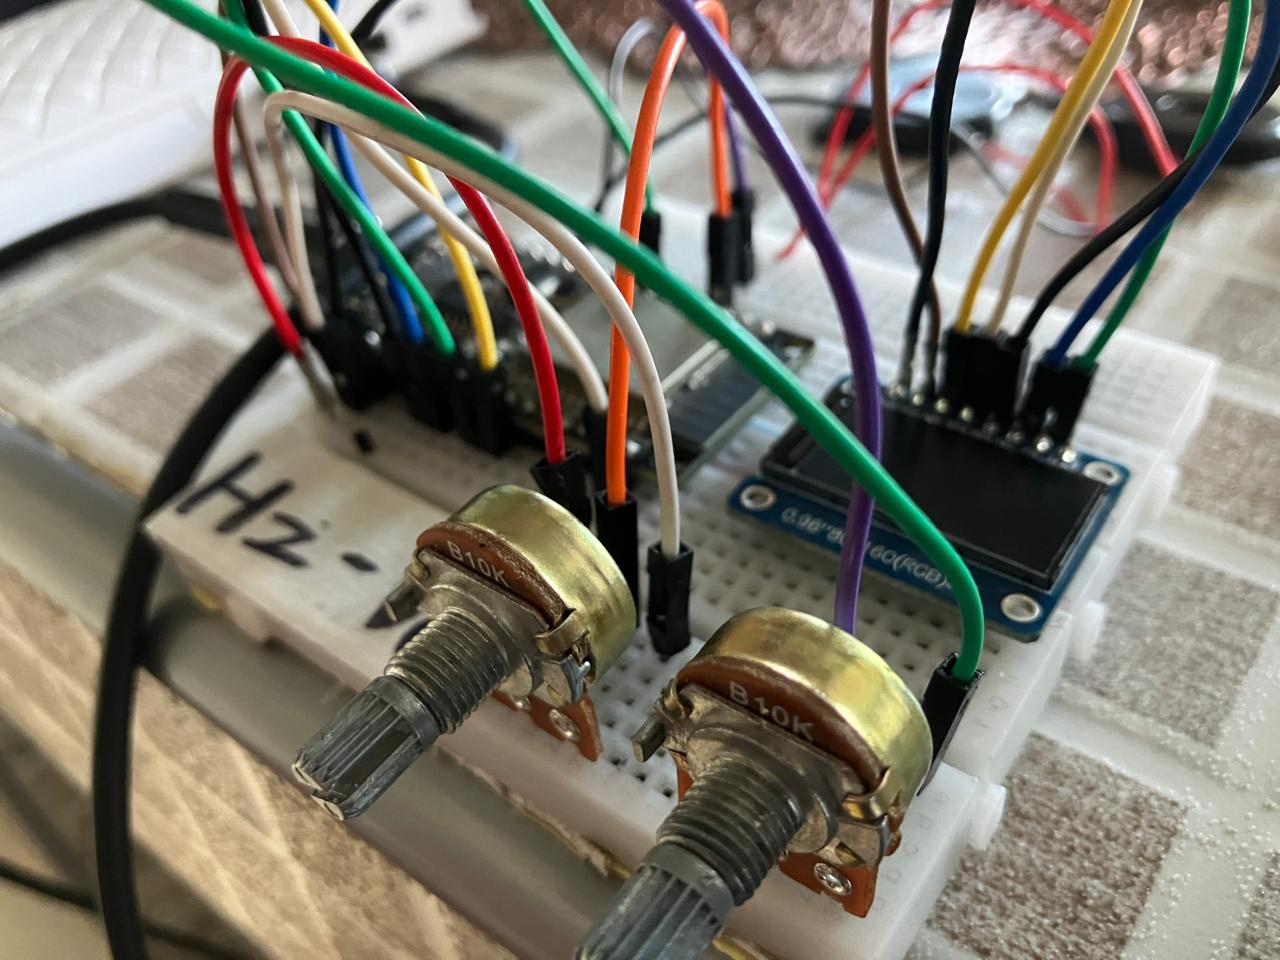
\includegraphics[width=\linewidth]{imagenes/50bf0c18-4558-440c-be7b-23011baf005c.jpeg}       
    \end{figure}
\end{itemize}

\subsection{Sistemas de Aplicación Acústica}

La aplicación de las ondas sonoras en el cultivo de plantas puede requerir sistemas de entrega más sofisticados, que aseguren que el sonido se propague de manera uniforme en el entorno de crecimiento:

\begin{itemize}
    \item \textbf{Holografia ultrasonica:}
    
    \item \textbf{Sistemas de Sonificación en Invernaderos:} La integración de tecnologías acústicas en invernaderos representa una forma innovadora de optimizar el crecimiento de las plantas. Estos sistemas pueden aplicar ondas sonoras de manera continua o intermitente, dependiendo de las necesidades específicas de las plantas, ayudando a maximizar el rendimiento y la calidad de los cultivos.
\end{itemize}

\subsection{Sensores y Monitoreo Acústico}

Para evaluar el impacto del sonido en las plantas, es esencial contar con dispositivos de monitoreo que midan la respuesta de las mismas a las ondas sonoras:

\begin{itemize}
    \item \textbf{Sensores de Crecimiento:} Estos dispositivos miden parámetros como la tasa de crecimiento, la elongación de las raíces y el desarrollo foliar, lo que permite correlacionar estos cambios con las frecuencias sonoras aplicadas. Sensores ópticos y de proximidad son comunes en estas aplicaciones.

    \item \textbf{Micrófonos de Alta Sensibilidad:} Se utilizan para capturar los sonidos emitidos por las plantas, que pueden ser indicativos de su estado de estrés o salud. Estos micrófonos pueden ayudar a entender cómo responden las plantas a diferentes condiciones acústicas.
    \begin{figure}[!h]
        \centering
        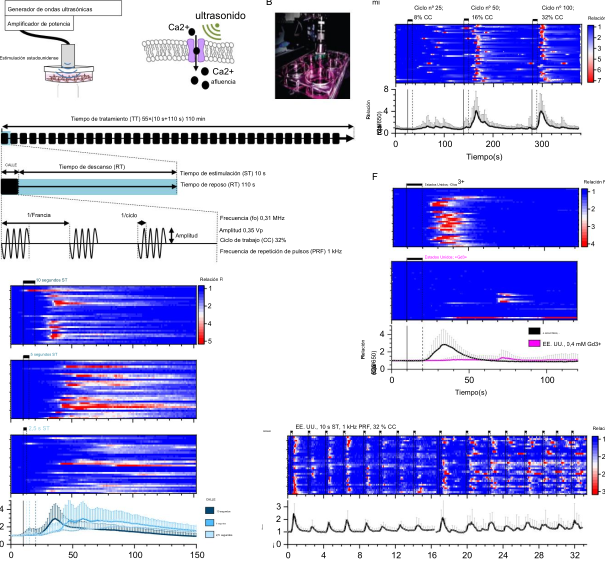
\includegraphics[width=\linewidth]{imagenes/Captura desde 2024-09-25 22-49-42.png}       
    \end{figure}
\end{itemize}

\subsection{Software de Análisis Acústico}

El desarrollo de software especializado es fundamental para analizar los datos obtenidos de los dispositivos acústicos:

\begin{itemize}
    \item \textbf{Análisis de Frecuencias:} Herramientas de software permiten descomponer los sonidos en sus componentes de frecuencia, facilitando la identificación de las frecuencias que tienen el mayor efecto sobre las plantas. Esto puede incluir el uso de espectrogramas y análisis de Fourier.
    \begin{figure}[!h]
        \centering
        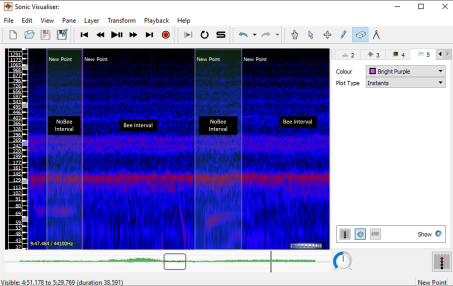
\includegraphics[width=\linewidth]{imagenes/Captura desde 2024-09-25 22-52-15.png}       
    \end{figure}
    \item \textbf{Modelado y Simulación:} Con la ayuda de software de modelado, se pueden simular diferentes escenarios acústicos para predecir cómo variaciones en la frecuencia, la amplitud y la duración del sonido podrían afectar el crecimiento y desarrollo de las plantas en entornos reales.
\end{itemize}

\subsection{posibles innovaciones Futuras}

El futuro del desarrollo de tecnologías y dispositivos acústicos en la sonobiología se presenta prometedor. Algunas áreas de innovación incluyen:

\begin{itemize}
    \item \textbf{Dispositivos Portátiles:} La creación de dispositivos acústicos portátiles podría permitir a los agricultores aplicar sonido en campos abiertos, haciendo accesibles los beneficios de la sonogenética en una escala más amplia.
    
    \item \textbf{Inteligencia Artificial y Aprendizaje Automático:} La integración de IA en el análisis de datos acústicos puede ayudar a identificar patrones complejos en las respuestas de las plantas al sonido, optimizando así las condiciones de cultivo de manera más eficiente.
    
    \item \textbf{Sistemas Híbridos:} Combinando tecnologías acústicas con otros métodos de cultivo, como hidroponía o aeroponía, se podrían maximizar los beneficios del sonido en ambientes controlados, mejorando la producción agrícola de manera sostenible.
\end{itemize}

El desarrollo continuo de tecnologías y dispositivos acústicos es esencial para avanzar en la comprensión de la sonobiología y su aplicación práctica en la agricultura. A medida que se desarrollen nuevas innovaciones, es probable que surjan más oportunidades para aprovechar el sonido en la mejora de los cultivos y la sostenibilidad agrícola.

\section{Posibles Mejoras Técnicas}

El avance en la sonogenética y su aplicación en la agricultura plantea una serie de oportunidades para la mejora técnica de los métodos y dispositivos utilizados. A continuación se presentan algunas áreas clave donde se pueden realizar mejoras:

\subsection{Optimización de Frecuencias Sonoras}

La identificación y utilización de frecuencias sonoras específicas que maximizan la respuesta positiva en las plantas es crucial. Algunas estrategias incluyen:

\begin{itemize}
    \item \textbf{Investigación de Frecuencias Óptimas:} Realizar estudios sistemáticos para identificar las frecuencias más efectivas para diferentes tipos de plantas y condiciones ambientales. Esto puede incluir pruebas en diferentes etapas de desarrollo y condiciones de estrés.
    
    \item \textbf{Desarrollo de Protocolos Personalizados:} Crear protocolos personalizados basados en las necesidades específicas de cada cultivo, utilizando la investigación sobre la respuesta a frecuencias sonoras para diseñar tratamientos acústicos más efectivos.
\end{itemize}

\subsection{Mejora de Dispositivos Acústicos}

Los dispositivos acústicos utilizados en la sonogenética deben ser adaptados y mejorados para maximizar su efectividad:

\begin{itemize}
    \item \textbf{Tecnología de Sonido Direccional:} Desarrollar sistemas que puedan dirigir el sonido de manera más eficiente a las áreas deseadas, asegurando que el estímulo acústico llegue efectivamente a las plantas objetivo.

    \item \textbf{Sensores Integrados:} Incorporar sensores que monitoricen el estado de las plantas en tiempo real, permitiendo ajustes automáticos en los parámetros acústicos según la respuesta de las plantas a los estímulos.
\end{itemize}

\subsection{3Integración con Tecnologías de Agricultura de Precisión}

La sonogenética puede beneficiarse enormemente de la integración con otras tecnologías modernas en la agricultura:

\begin{itemize}
    \item \textbf{Análisis de Datos:} Implementar herramientas de análisis de datos para interpretar las respuestas de las plantas a las exposiciones acústicas, lo que permite una mejor toma de decisiones y una adaptación rápida de las estrategias.

    \item \textbf{Sistemas de Riego Inteligente:} Combinar técnicas de sonido con sistemas de riego inteligente para optimizar el uso de recursos hídricos en función de la respuesta de las plantas al sonido.
\end{itemize}

\subsection{Escalabilidad y Accesibilidad}

Para que la sonogenética tenga un impacto significativo en la agricultura, es fundamental que las técnicas sean escalables y accesibles:

\begin{itemize}
    \item \textbf{Desarrollo de Equipos de Bajo Costo:} Investigar y desarrollar tecnologías que sean accesibles económicamente para pequeños agricultores, permitiendo que los beneficios de la sonogenética se extiendan a una amplia gama de productores.

    \item \textbf{Capacitación y Educación:} Proveer programas de capacitación para agricultores sobre cómo implementar y beneficiarse de la sonogenética, asegurando que puedan adoptar estas tecnologías de manera efectiva.
\end{itemize}

\subsection{Colaboración Interdisciplinaria}

Fomentar la colaboración entre diferentes disciplinas puede llevar a innovaciones significativas en la sonogenética:

\begin{itemize}
    \item \textbf{Investigación Interdisciplinaria:} Promover la colaboración entre biólogos, ingenieros, agrónomos y expertos en acústica para desarrollar un enfoque más integral y efectivo para la aplicación de la sonogenética.

    \item \textbf{Proyectos de Investigación Conjunta:} Iniciar proyectos de investigación conjunta que exploren nuevas aplicaciones y técnicas, integrando conocimientos y experiencias de diversas áreas.
\end{itemize}

La implementación de estas mejoras técnicas no solo puede aumentar la efectividad de la sonogenética, sino que también puede abrir nuevas avenidas para la innovación agrícola y contribuir a la sostenibilidad en la producción de alimentos.

\section{Futuras Líneas de Investigación}

A medida que la sonobiología y la sonogenética continúan evolucionando, surgen diversas áreas de investigación que podrían contribuir a un mayor entendimiento y aplicación de estas disciplinas en la agricultura y otros campos. A continuación, se presentan algunas líneas de investigación prometedoras:

\subsection{Mecanismos de Acción a Nivel Molecular}

La comprensión detallada de los mecanismos moleculares subyacentes a la sonogenética es fundamental para su avance. Algunas áreas de enfoque incluyen:

\begin{itemize}
    \item \textbf{Estudio de Genes Específicos:} Identificar y caracterizar genes que son regulados por estímulos sonoros, así como sus funciones en el crecimiento y desarrollo de las plantas.
    
    \item \textbf{Interacciones con Hormonas Vegetales:} Investigar cómo las ondas sonoras afectan las rutas hormonales en las plantas y cómo estas interacciones pueden influir en el crecimiento y la respuesta a estrés.
\end{itemize}

\subsection{Efectos a Largo Plazo del Sonido en Plantas}

Se necesita más investigación sobre los efectos a largo plazo de la exposición continua a diferentes frecuencias sonoras en las plantas:

\begin{itemize}
    \item \textbf{Estudios de Ciclos de Vida:} Evaluar cómo las exposiciones acústicas afectan las etapas críticas del ciclo de vida de las plantas, incluyendo la germinación, crecimiento, reproducción y senescencia.
    
    \item \textbf{Impacto en la Biodiversidad:} Investigar cómo la sonogenética puede influir en la biodiversidad de especies de plantas en un ecosistema y su interacción con otros organismos.
\end{itemize}

\subsection{Aplicaciones en Cultivos de Interés Económico}

La sonogenética tiene el potencial de revolucionar cultivos específicos con un alto valor económico:

\begin{itemize}
    \item \textbf{Optimización de Cultivos:} Investigar el uso de sonogenética en cultivos comerciales, como frutas y verduras, para mejorar rendimientos y calidad.
    
    \item \textbf{Resiliencia a Cambios Climáticos:} Estudiar cómo la sonogenética puede aumentar la resiliencia de los cultivos ante condiciones climáticas extremas, como sequías o inundaciones.
\end{itemize}

\subsection{Desarrollo de Tecnologías Innovadoras}

La innovación tecnológica es crucial para maximizar los beneficios de la sonobiología:

\begin{itemize}
    \item \textbf{Sistemas de Sonido Inteligentes:} Desarrollar dispositivos acústicos avanzados que integren inteligencia artificial para ajustar dinámicamente las frecuencias y patrones de sonido basados en la respuesta de las plantas.
    
    \item \textbf{Monitoreo Remoto:} Implementar tecnologías de monitoreo remoto para evaluar en tiempo real la efectividad de las aplicaciones sonoras en diversas condiciones ambientales.
\end{itemize}




\section{Conclusiones}
La sonobiología y la sonogenética ofrecen nuevas perspectivas para la agricultura. Al aprovechar las propiedades del sonido, podemos no solo mejorar la producción agrícola, sino también contribuir a la sostenibilidad del medio ambiente. La investigación en este campo está en sus primeras etapas, pero los resultados son prometedores y abren un abanico de posibilidades para el futuro de la agricultura.

\section*{Bibliografía}

\begin{thebibliography}{99}

\bibitem{vicient2017}
Carlos M. Vicient,
\textit{The effect of frequency-specific sound signals on the germination of maize seeds},
BMC Research Notes \textbf{10} (2017): 323. doi: \url{10.1186/s13104-017-2643-4}.

\bibitem{collins2001effect}
Margaret E. Collins and John E. K. Foreman,
\textit{The effect of sound on the growth of plants},
Canadian Acoustics \textbf{29} (2001): 3--8.

\bibitem{altuntas2019tomato}
Onder Altuntas and Huseyin Ozkurt,
\textit{The assessment of tomato fruit quality parameters under different sound waves},
Journal of Food Science and Technology \textbf{56} (2019): 2186--2194. doi: \url{10.1007/s13197-019-03701-0}.

\bibitem{ozkurt2016}
Halil Ozkurt and Ozlem Altuntas,
\textit{The Effect of Sound Waves at Different Frequencies upon the Plant Element Nutritional Uptake of Snake Plant (Sansevieria Trifasciata) Plants},
Indian Journal of Science and Technology \textbf{9} (2016): 1--5. doi: \url{10.17485/ijst/2016/v9i48/54716}.

\bibitem{rakic2021}
V. Rakić and N. Poklar Ulrih,
\textit{Influence of pH on color variation and stability of cyanidin and cyanidin 3-O-β-glucopyranoside in aqueous solution},
CyTA - Journal of Food \textbf{19} (2021): 174--182. doi: \url{10.1080/19476337.2021.1874539}.

\bibitem{sorum2024tension}
Benjamin Sorum, Tyler Docter, Valerio Panico, et al.,
\textit{Tension activation of mechanosensitive two-pore domain K+ channels TRAAK, TREK-1, and TREK-2},
Nature Communications \textbf{15} (2024): 3142. doi: \url{10.1038/s41467-024-47208-5}.

\bibitem{khait2023sounds}
Itzhak Khait, Ohad Lewin-Epstein, Raz Sharon, Nir Sade, Yossi Yovel, and Lilach Hadany,
\textit{Sounds emitted by plants under stress are airborne and informative},
Cell \textbf{186} (2023): 1328--1336.e10. doi: \url{10.1016/j.cell.2023.02.020}.

\bibitem{agromining2021}
Antony van der Ent, Alan J.M. Baker, Guillaume Echevarria, Marie-Odile Simonnot, and Jean Louis Morel (Eds.),
\textit{Agromining: Farming for Metals - Extracting Unconventional Resources Using Plants}, 2nd ed. (2021). Springer.

\bibitem{medina2024rare}
Hassay Lizeth Medina-Díaz, Francisco Javier López-Bellido, Jacinto Alonso-Azcárate, Francisco Jesús Fernández-Morales, and Luis Rodríguez,
\textit{Can rare earth elements be recovered from abandoned mine tailings by means of electrokinetic-assisted phytoextraction?},
Environmental Science and Pollution Research \textbf{31} (2024): 26747--26759. doi: \url{10.1007/s11356-024-32759-3}.

\bibitem{souza2024nitrate}
C. de Souza Junior and F.A. Monteiro,
\textit{Nitrate fertilization enhances manganese phytoextraction in Tanzania guinea grass: a novel hyperaccumulator plant?},
Environmental Science and Pollution Research \textbf{31} (2024): 9661--9670. doi: \url{10.1007/s11356-023-31548-8}.

\bibitem{katz2022genetic}
M. Katz,
\textit{Genetic Methods for Cellular Manipulation in \textit{C. elegans}},
in G. Haspel and A.C. Hart (Eds.), \textit{C. elegans}, Methods in Molecular Biology \textbf{2468} (2022): 71--91. Humana. doi: \url{10.1007/978-1-0716-2181-3_4}.

\bibitem{sorum2024activacion}
Ben Sorum, Trevor Docter, Vincent Panico, Robert A. Rietmeijer, and Stephen G. Brohawn,
\textit{Activación por tensión de los canales de K+ de dominio de dos poros mecanosensibles TRAAK, TREK-1 y TREK-2},
Nature Communications (2024). doi: \url{10.1038/s41467-024-47208-5}.

\bibitem{liao2021longitud}
Defei Liao, Ming Yen Hsiao, Gaoming Xiang, and Pei Zhong,
\textit{Longitud óptima del pulso de insonificación para la activación de Piezo1 y la respuesta del calcio intracelular},
Scientific Reports \textbf{11} (2021): 709. doi: \url{10.1038/s41598-020-78553-2}.

\bibitem{hassanien2014avances}
Reda Hassanien, Bao Ming Li, et al.,
\textit{Avances en los efectos de las ondas sonoras en las plantas},
Revista de Agricultura Integrativa (2014), Febrero. doi: \url{10.1016/S2095-3119(13)60492-X}.

\bibitem{khait2023sonidos}
Itzhak Khait, Ohad Lewin-Epstein, Raz Grabación, Nir Sade, Yossi Yovel, and Lilach Hadany,
\textit{Los sonidos emitidos por las plantas bajo estrés son transmitidos por el aire e informativos},
Cell \textbf{186} (2023): 1328--1336. doi: \url{10.1016/j.cell.2023.03.009}.

\bibitem{parlakova2021ultra}
F. Parlakova Karagöz and A. Dursun,
\textit{Ultra-Sonic Sound Applications Used in Seed Viability, Seedling Growth and Plant Development of Ornamentals},
Journal of the Institute of Science and Technology \textbf{11}, Special Issue (2021): 3416--3428. doi: \url{10.21597/jist.1027370}.

\bibitem{zapien2019generacion}
José Manuel Zapien-Rodríguez, Bianca Azucena Solorio-De Jesús, Juan Carlos Ballesteros-Pacheco, and Frida Libertad Núñez-Ayala,
\textit{Generación Eléctrica a Partir de la Fotosíntesis Natural; ¿Una Realidad Escalable?},
Revista de Energías Renovables \textbf{3} (2019): 1--6. doi: \url{10.35429/JRE.2019.10.3.1.6}.

\end{thebibliography}


\end{document}
